\documentclass[a4paper,11pt]{article}
\usepackage{graphicx}

\begin{document}

\begin{flushright}

\vspace{1.1cm}

%Put ISR Title
{\bf\Huge Problem Set 1}

\rule{0.25\linewidth}{0.5pt}

\vspace{0.5cm}
%Put Authors
Justin Ely
\linebreak
\newline
%Put Author's affiliations
\footnotesize{AST622 University of Maryland College Park, MD\\}
\vspace{0.5cm}
% Date here below
22 February, 2012
\end{flushright}

\noindent\rule{\linewidth}{1.0pt}
\section*{1) Conservation of Energy}
\subsection*{a] Energy continuity equation}
To derive the energy continuity equation from the Friedmann equations we will start with:
\begin{eqnarray}
\ddot{a}=\frac{-4\pi G}{3}(\rho+3\frac{p}{c^2})a \\
\dot{a}^2=-kc^2+\frac{8 \pi G}{3} \rho a^2
\end{eqnarray}

Multiply both sides of (1) by $\dot{a}$ and eliminating $\ddot{a}$:
\begin{equation}
\frac{1}{2}\frac{d}{dt}\dot{a}^2=\frac{-4\pi G}{3}(\rho a \dot{a}+3\frac{p}{c^2} a \dot{a})
\end{equation}

Then combining (2) and (3):
\begin{eqnarray}
\frac{d}{dt}(-kc^2+\frac{8 \pi G \rho a^2}{3})= \frac{-8 \pi G}{3}(\rho-\frac{3p}{c^2})a \dot{a} \nonumber \\
\nonumber \\
\frac{d}{dt}\frac{-8 \pi G}{c^2}+\frac{d}{dt}\frac{-8 \pi G \rho a^2}{3}                         \nonumber \\
\nonumber \\
\frac{-8 \pi G a^2}{3} \frac{d}{dt}\rho= \frac{-8 \pi G a^2}{3}(\rho - \frac{3p}{c^2}a \dot{a})    \nonumber \\
\nonumber \\
\dot{\rho}=-\rho H + \frac{3p}{c^2}H                                  \nonumber \\
\nonumber \\
\dot{\rho}+H(\rho-\frac{3p}{c^2})=0 
\nonumber \\
\end{eqnarray}

*(Note this solution isn't correct, I couldn't get rid of the factor of 3 in the final continuity equation)

\subsection*{b] First law of thermodynamics}
The first law of thermodynamics, $dU=dQ-pdV$, states that the energy of an isolated system is constant using internal energy, heat, and work.  The continuity equation states the same thing; that the sum of acceleration of the universe, mass energy, and kinetic energy is a constant.  

\subsection*{c] Conservation of energy}
The continuity equation says that energy is conserved in the universe as a whole, as it can be taken for an isolated system in which no energy can be added or subtracted.  In the hypothetical example of a universe that contains only photons, the decrease in energy of the photons as the universe expands would need to be accompanied by an increase in the energy of the acceleration.  

\subsection*{d] Conservation of energy in the universe}
If the expansion of the universe is adiabatic, then total energy is conserved.  This needs to include the energy of the expansion, as energy is being lost from the matter and relativistic componenents of the universe.  I'm not completely sure why N-Body cosmological simulations do not conserve energy.  It could be related to the algorithm being used in that some methods do not conserve energy, or perhaps N-Body simulations only account for dust matter and expansion and do not account for relativistic matter.

\section*{2) Matter Dominated Models}
\begin{eqnarray}
%\dot{a}=\frac{8 \pi G}{3 c^2} \Sigma \epsilon_{w,0} a^{-1-3w}-\frac{k c^2}{R_0^2}
\frac{H^2}{H_0^2}=\frac{\Omega_{r,0}}{a^4}+\frac{\Omega_{m,0}}{a^3}+\Omega_{\Lambda,0}+\frac{1-\Omega_0}{a^2}
\end{eqnarray}

The Friedmann equation for a multi-component universe is given above.  For a matter dominated universe, the radiation and expansion terms are 0, so $\Omega_{m}$ is the only component.  This yields the equation below, which can be solved for a(t).

\begin{eqnarray}
\frac{H^2}{H_0^2}=\frac{\Omega_{0}}{a^3}+\frac{1-\Omega_0}{a^2} \nonumber \\
H=\frac{\dot{a}}{a}  \nonumber \\
\frac{\dot{a}^2}{H_0^2}=\frac{\Omega_{0}}{a}+(1-\Omega_0) \nonumber \\
H_0t=\int\limits_0^a \frac{da}{[\frac{\Omega_{0}}{a}+(1-\Omega_0)]^{1/2}}
\end{eqnarray}

\subsection*{a] a(t) for closed universe}
(6) has a solution when $\Omega_o > 1$, representing a closed universe, given by:
\begin{equation}
a(\theta)=\frac{1}{2}\frac{\Omega_o (1-cos(\theta))}{\Omega_0-1}
\end{equation}

\subsection*{b] a(t) for open universe}
Open universes,$\Omega_o < 1$, also has a solution to (6) given by:
\begin{equation}
a(\theta)=\frac{1}{2}\frac{\Omega_o (cosh(\theta)-1)}{1-\Omega_0}
\end{equation}

\subsection*{c] Evolution of a(t)}
Figure 1 shows the evolution of a(t) vs. time for both a closed and open universe.  It is clearly evident from the plot that a closed universe will collapse back on itself after a time period determined by $\Omega$, while an open universe will continue to expand forever.  This is consistant with what we have learned about the various cosomological models.
\begin{figure}[h!]
\begin{center}
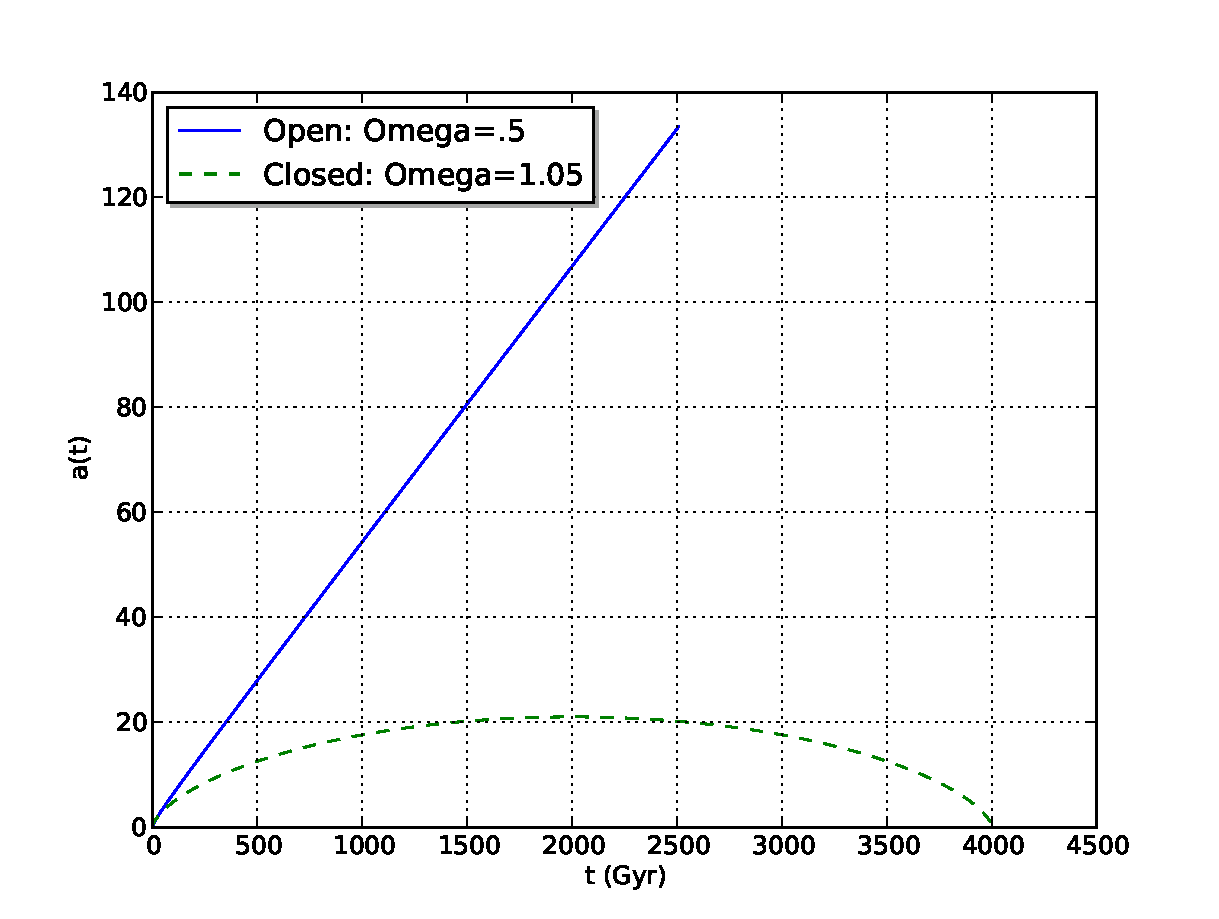
\includegraphics[scale=.7]{two_c.pdf}
\caption{Evolution of a(t) for open and closed universes.}
\end{center}
\end{figure}


\subsection*{d] Age of the universe}
The age of the universe for various models can be determined by finding where $a(t)=1$ for each model.  As can be seen in Figure 2, the current age of the universe(when a(t)=1) gets smaller for larger values of omega.  This makes sense as a higher value of $\Omega$ means a slower expansion of the universe, so it would have to have been expanding for much longer to reach the present size.  
\begin{figure}[h!]
\begin{center}
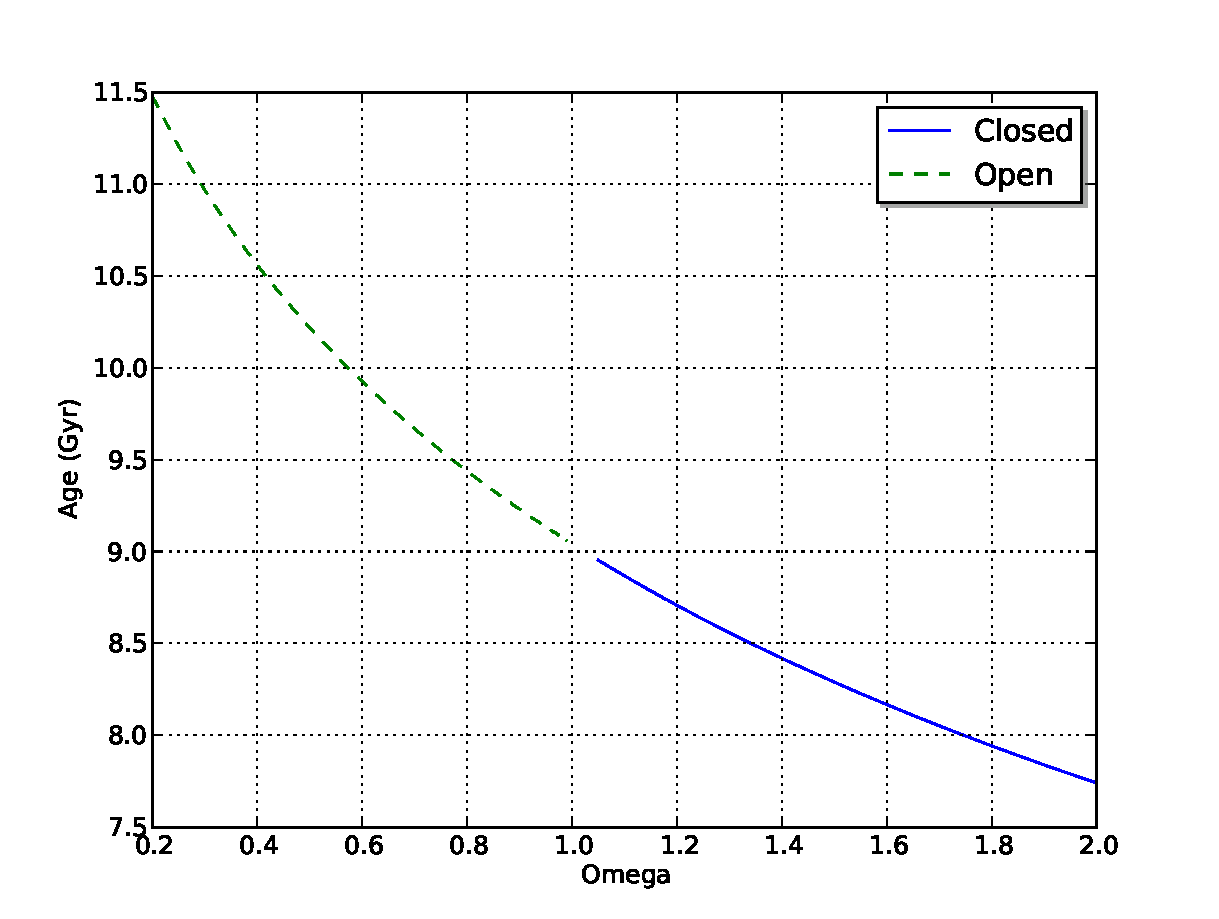
\includegraphics[scale=.7]{two_d.pdf}
\caption{Age of the universe vs. Omega.}
\end{center}
\end{figure}


%\section*{3}
%\subsection*{a}
%\begin{eqnarray}
%d_A=\frac{r(x)}{1+z}  \\
%r(x)=\frac{sinh(\sqrt{\Omega_k}H_0 x}{H_0 \sqrt{\|{\Omega_k}\|}}
%\end{eqnarray}

%\subsection*{b}
%\begin{eqnarray}
%m-M=-5+5log(d_L) \\
%d_L=\frac{2c}{H_0 \Omega_0^2}(\Omega_0 z +(\Omega_0 -z)[-1+(\Omega_0 z+1)^{\frac{1}{2}}])
%\end{eqnarray}


\end{document}
